\section{An Introduction to Differential Equations} \label{S:6.6.DEIntro}

\begin{goals}
\item What is a differential equation and what kinds of information can it tell us?
\item How do differential equations arise in the world around us?
\item What do we mean by a solution to a differential equation?
\item What is a slope field and how can we use a slope field to obtain qualitative information about the solutions of a differential equation?
\item What are stable and unstable equilibrium solutions of an autonomous differential equation? 
\end{goals} 

%---------------------------------------------
% SUBSECTION INTRODUCTION
%---------------------------------------------
\subsection*{Introduction}

In previous chapters, we have seen that a function's derivative tells us the rate at which the function is changing.  More recently, the Fundamental Theorem of Calculus helped us to determine the total change of a function over an interval when we know the function's rate of change.  For instance, an object's velocity tells us the rate of change of that object's position.  By integrating the velocity over a time interval, we may determine by how much the position changes over that time interval.  In particular, if we know where the object is at the beginning of that interval, then we have enough information to accurately predict where it will be at the end of the interval. 

In this section, we will introduce the concept of \emph{differential equations} and explore this idea in more depth.  Simply said, a differential equation is an equation that provides a description of a function's derivative, which means that it tells us the function's rate of change.  Using this information, we would like to learn as much as possible about the function itself.  For instance, we would ideally like to have an algebraic description of the function.  

\begin{pa} \label{PA:7.1}
The position of a moving object is given by the function $s(t)$, where $s$ is measured in feet and $t$ in seconds.  We determine that the velocity is $v(t) = 4t + 1$ feet per second. 
\ba
\item How much does the position change over the time interval   $[0,4]$?

\item Does this give you enough information to determine $s(4)$, the position at time $t=4$?  If so, what is $s(4)$?  If not, what additional information would you need to know to determine $s(4)$?

\item Suppose you are told that the object's initial position $s(0) = 7$.  Determine $s(2)$, the object's position $2$ seconds later. 

\item If you are told instead that the object's initial position is $s(0) = 3$, what is $s(2)$?

\item If we only know the velocity $v(t)=4t+1$, is it possible that the object's position at all times is $s(t) = 2t^2 + t - 4$?  Explain how you know.

\item Are there other possibilities for $s(t)$?  If so, what are they?  

\item If, in addition to knowing the velocity function is $v(t) = 4t+1$, we know the initial position $s(0)$, how many possibilities are there for $s(t)$?
\ea
\end{pa} 
\afterpa
 %PREVIEW 

%-------------------------------------------------------------
% SUBSECTION DIFFERENTIAL EQUATIONS
%-------------------------------------------------------------
\subsection*{What is a differential equation?} \index{differential equation} 

A differential equation is an equation that describes the derivative, or derivatives, of a function that is unknown to us.  For instance, the equation
$$ \frac{dy}{dx} = x \sin(x) $$
is a differential equation since it describes the derivative of a function $y(x)$ that is unknown to us.

As many important examples of differential equations involve quantities that change in time, the independent variable in our discussion will frequently be time $t$. For instance, in the preview activity, we considered the differential equation
$$ \frac{ds}{dt} = 4t + 1. $$
Knowing the velocity and the starting position of the object, we were able to find the position at any later time.

Because differential equations describe the derivative of a function, they give us information about how that function changes.  Our goal will be to take this information and use it to predict the value of the function in the future; in this way, differential equations provide us with something like a crystal ball.

Differential equations arise frequently in our every day world.  For instance, you may hear a bank advertising:

\begin{quote}{\em Your money will grow at a 3\% annual interest rate with us.}\end{quote}

This innocuous statement is really a differential equation.  Let's translate:  $A(t)$ will be amount of money you have in your account at time $t$.  On one hand, the rate at which your money grows is the derivative $dA/dt$.  On the other hand, we are told that this rate is $0.03 A$.  This leads to the differential equation
$$ \frac{dA}{dt} = 0.03 A. $$

This differential equation has a slightly different feel than the previous equation $\frac{ds}{dt} = 4t+1$.  In the earlier example, the rate of change depends only on the independent variable $t$, and we may find $s(t)$ by integrating the velocity $4t+1$.   In the banking example, however, the rate of change depends on the dependent variable $A$, so we'll need some new techniques in order to find $A(t)$.  

\begin{activity} \label{A:6.6.1}  Express the following statements as   differential equations.  In each case, you will need to introduce notation to describe the important quantities in the statement so be sure to clearly state what your notation means.
\ba
	\item The population of a town grows at an annual rate of $1.25$\%. 
        \item A radioactive sample loses $5.6$\% of its mass every day.
        \item You have a bank account that earns $4$\% interest every year.  At the same time, you withdraw money continually from the account at the rate of \$$1000$ per year.
        \item A cup of hot chocolate is sitting in a $70^\circ$ room. The temperature of the hot chocolate cools by $10$\% of the difference between the hot chocolate's temperature and the room temperature every minute.
        \item A can of cold soda is sitting in a $70^\circ$ room. The temperature of the soda warms at the rate of $10$\% of the difference between the soda's temperature and the room's temperature every minute.
\ea
\end{activity}
\begin{smallhint}
\ba
	\item Small hints for each of the prompts above.
\ea
\end{smallhint}
\begin{bighint}
\ba
	\item Big hints for each of the prompts above.
\ea
\end{bighint}
\begin{activitySolution}
\ba
	\item Solutions for each of the prompts above.
\ea
\end{activitySolution}
\aftera %ACTIVITY

Differential equations may be classified based on certain characteristics they may possess.  Indeed, you may see many different types of differential equations in a later course in differential equations.  For now, we would like to introduce a few terms that are used to describe differential equations.

A {\em first-order} differential equation\index{differential equation!first order} is one in which only the first derivative of the function occurs.  For this reason,
$$ \frac{dv}{dt} = 1.5-0.5v $$
is a first-order equation while
$$ \frac{d^2 y}{dt^2} = -10y $$
is a second-order equation.

A differential equation is {\em autonomous}\index{autonomous} \index{differential equation!autonomous} if the independent variable does not  appear in the description of the derivative.  For instance,
$$ \frac{dv}{dt} = 1.5-0.5v $$
is autonomous because the description of the derivative $dv/dt$ does not depend on time.   The equation
$$ \frac{dy}{dt} = 1.5t - 0.5y, $$
however, is not autonomous.

%-------------------------------------------------------------------
% SUBSECTION DE IN THE WORLD AROUND US
%-------------------------------------------------------------------
\subsection*{Differential equations in the world around us}

As we have noted, differential equations give a natural way to describe phenomena we see in the real world.  For instance, physical principles are frequently expressed as a description of how a quantity changes.  A good example is Newton's Second Law, an important physcial principle that says:  

\begin{quote} {\em The product of an object's mass and acceleration equals the force applied to it.} \end{quote}

For instance, when gravity acts on an object near the earth's surface, it exerts a force equal to $mg$, the mass of the object times the gravitational constant $g$.  We therefore have 
\begin{eqnarray*} 
ma & = & mg, \ \mbox{or} \\
\quad \frac{dv}{dt} & = & g,
\end{eqnarray*}
where $v$ is the velocity of the object, and $g = 9.8$ meters per second squared.  Notice that this physical principle does not tell us what the object's velocity is, but rather how the object's velocity changes.  

\begin{activity} \label{A:6.6.2}  
Shown are two graphs depicting the velocity of falling objects.  One is the velocity of a skydiver, while the other is the velocity of a meteorite entering the Earth's atmosphere.

\ba
	\item Begin with the skydiver's velocity and use the given graph to measure the rate of change $dv/dt$ when the velocity is $v=0.5, 1.0, 1.5,
          2.0$, and $2.5$.  Plot your values on the graph below.  You
          will want to think carefully about this:  you are plotting
          the derivative $dv/dt$ as a function of {\em velocity}.

          \begin{center}
            \scalebox{0.65}{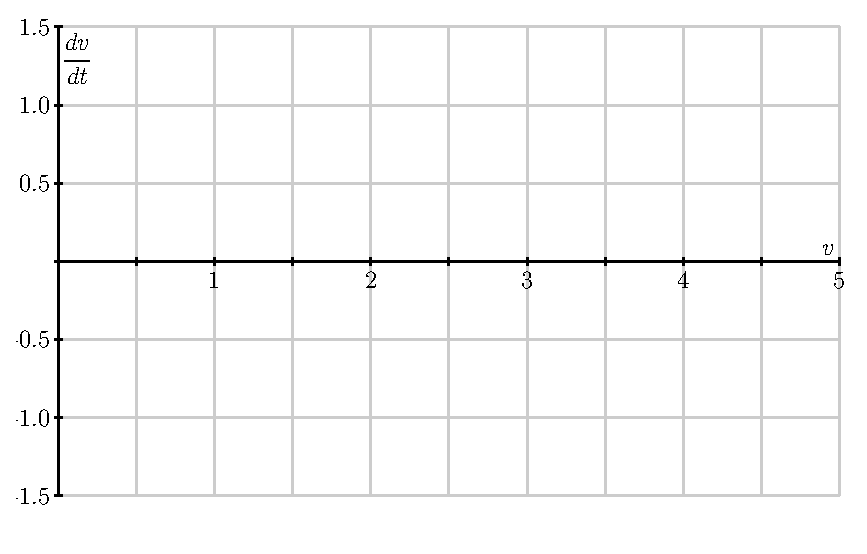
\includegraphics{figures/7_1_dataplot.eps}}
          \end{center}
        \item Now do the same thing with the meteorite's velocity:
          use the given graph to measure the rate of change $dv/dt$ when the velocity is
          $v=3.5,4.0,4.5$, and $5.0$.  Plot your values on the graph
          above. 
        \item You should find that all your points lie on a line.
          Write the equation of this line being careful to use proper
          notation for the quantities on the horizontal and vertical
          axes.
        \item The relationship you just found is a differential
          equation.  Write a complete sentence that explains its
          meaning. 
        \item By looking at the differential equation, determine the
          values of the velocity for which the velocity 
          increases.
        \item By looking at the differential equation, determine the
          values of the velocity for which the velocity 
          decreases.
        \item By looking at the differential equation, determine the
          values of the velocity for which the velocity 
          remains constant.

\ea
\end{activity}

\begin{marginfigure}[-6cm]
\begin{center}
\subfloat[Skydiver's velocity]{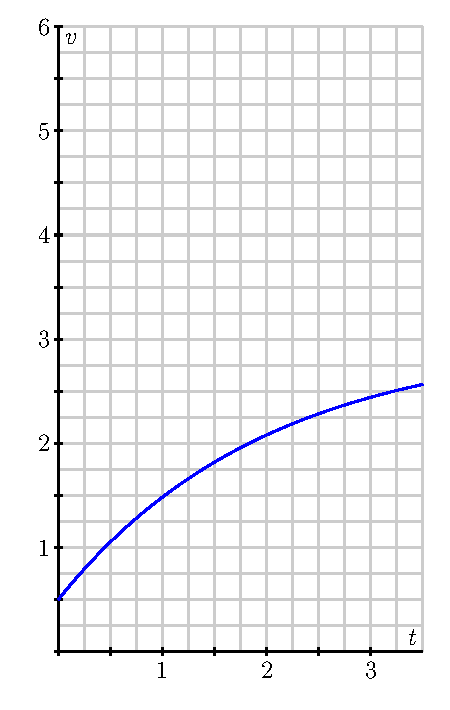
\includegraphics[scale=.75]{figures/7_1_activity_0.eps}}

\subfloat[Meteorite's velocity]{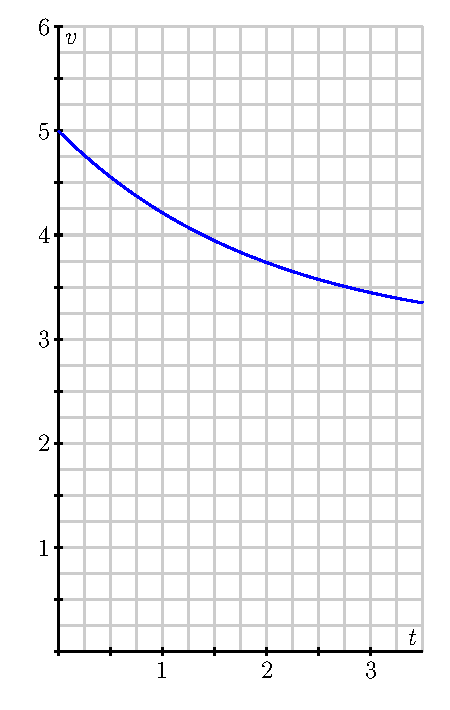
\includegraphics[scale=.75]{figures/7_1_activity_1.eps}}
\end{center}
\caption{Graphs of velocities used in Activity~\ref{A:6.6.2}.}
\end{marginfigure}


\begin{smallhint}
\ba
	\item Small hints for each of the prompts above.
\ea
\end{smallhint}
\begin{bighint}
\ba
	\item Big hints for each of the prompts above.
\ea
\end{bighint}
\begin{activitySolution}
\ba
	\item Solutions for each of the prompts above.
\ea
\end{activitySolution}
\aftera %ACTIVITY

The point of this activity is to demonstrate how differential equations model processes in the real world.  In this example, two factors are influencing the velocities:  gravity and wind resistance. The differential equation describes how these factors influence the rate of change of the objects' velocities.

%---------------------------------------------
% SUBSECTION SOLVING DE
%---------------------------------------------
\subsection*{Solving a differential equation} \index{differential equation!solution}

We have said that a differential equation is an equation that describes the derivative,  or derivatives, of a function that is unknown to us.  By a {\em   solution} to a differential equation, we mean simply a function that satisfies this description.

For instance, the first differential equation we looked at is 
$$ \frac{ds}{dt} = 4t+1, $$
which describes an unknown function $s(t)$.  We may check that $s(t) = 2t^2+t$ is a solution because it satisfies this description.  Notice that $s(t) = 2t^2+t+4$ is also a solution.

If we have a candidate for a solution, it is straightforward to check whether it is a solution or not.  Before we demonstrate, however, let's consider the same issue in a simpler context. Suppose we are given the equation $2x^2 - 2x = 2x+6$ and asked whether $x=3$ is a solution.  To answer this question, we could rewrite the variable $x$ in the equation with the symbol $\Box$:
$$ 2\Box^2 - 2\Box = 2\Box + 6. $$
To determine whether $x=3$ is a solution, we can investigate the value of each side of the equation separately when the value $3$ is placed in $\Box$ and see if indeed the two resulting values are equal.  Doing so, we observe that 
$$2\Box^2 - 2\Box = 2\cdot3^2 - 2\cdot3 = 12,$$
and
$$2\Box + 6 = 2\cdot3 + 6 = 12.$$
Therefore, $x=3$ is indeed a solution.

We will do the same thing with differential equations.  Consider the differential equation 
\begin{eqnarray*}
\frac{dv}{dt} & = & 1.5 - 0.5v, \ \mbox{or} \\
\quad \frac{d\Box}{dt} & = & 1.5 - 0.5\Box.
\end{eqnarray*}
Let's ask whether $v(t) = 3 - 2e^{-0.5t}$ is a solution\footnote{At this time, don't worry about why we chose this function;  we will learn techniques for finding solutions to differential equations soon enough.  }.  Using this formula for $v$, observe first that
$$\frac{dv}{dt} =  \frac{d\Box}{dt}  = \frac{d}{dt}[3 - 2e^{-0.5t}] = -2e^{-0.5t} \cdot (-0.5) = e^{-0.5t}$$
and
$$1.5 - 0.5v = 1.5 - 0.5\Box= 1.5 - 0.5(3 - 2e^{-0.5t}) = $$
$$1.5 - 1.5 + e^{-0.5t} = e^{-0.5t}.$$
Since $\frac{dv}{dt}$ and $1.5 - 0.5v$ agree for all values of $t$ when $v = 3-2e^{-0.5t}$, we have indeed
found a solution to the differential equation.

\begin{activity} \label{A:7.1.3}  Consider the differential equation 
$$
\frac{dv}{dt} = 1.5 - 0.5v.
$$
Which of the following functions are solutions of this differential equation?
\ba
	\item $v(t) = 1.5t - 0.25t^2$.
        \item $v(t) = 3 + 2e^{-0.5t}$.
        \item $v(t) = 3$.
        \item $v(t) = 3 + Ce^{-0.5t}$ where $C$ is any constant.
\ea
\end{activity}
\begin{smallhint}
\ba
	\item Small hints for each of the prompts above.
\ea
\end{smallhint}
\begin{bighint}
\ba
	\item Big hints for each of the prompts above.
\ea
\end{bighint}
\begin{activitySolution}
\ba
	\item Solutions for each of the prompts above.
\ea
\end{activitySolution}
\aftera %ACTIVITY

This activity shows us something interesting.  Notice that the differential equation has infinitely many solutions, which are parameterized by the constant $C$ in $v(t) = 3+Ce^{-0.5t}$.  In Figure~\ref{F:7.1.family}, we see the graphs of these solutions for a few values of $C$,  as labeled.

\begin{marginfigure}[3cm] % MARGIN FIGURE
\margingraphics{figures/7_1_family.eps}
\caption{The family of solutions to the differential equation $\frac{dv}{dt} = 1.5 - 0.5v$.} \label{F:7.1.family} 
\end{marginfigure}

Notice that the value of $C$ is connected to the initial value of the velocity $v(0)$, since $v(0) = 3+C$.  In other words, while the differential equation describes how the velocity changes as a function of the velocity itself, this is not enough information to determine the velocity uniquely:  we also need to know the initial velocity.  For this reason, differential equations will typically have infinitely many solutions, one corresponding to each initial value.  We have seen this phenomenon before, such as when given the velocity of a moving object $v(t)$, we were not able to uniquely determine the object's position unless we also know its initial position.

If we are given a differential equation and an initial value for the unknown function, we say that we have an {\em initial value problem.} For instance,
$$   \frac{dv}{dt} = 1.5-0.5v, \ v(0) = 0.5 $$
is an initial value problem.  In this situation, we know the value of $v$ at one time and we know how $v$ is changing.  Consequently, there should be exactly one function $v$ that satisfies the initial value problem.

%This demonstrates the following important general property of initial value problems.
%
%\concept{Initial Value Problems}{
%    Initial value problems that are ``well behaved'' have exactly one
%    solution, which exists in some interval around the initial point.
%} % end concept
%
%We won't worry about what ``well behaved'' means---it is a technical
%condition that will be satisfied by all the differential equations we
%consider. 

%---------------------------------------------
% SUBSECTION SLOPE FIELDS
%---------------------------------------------
\subsection{Slope Fields} \index{Slope Fields}

We may sketch the solution to an initial value problem if we know an appropriate collection of tangent lines.  Because we may use a given differential equation to determine the slope of the tangent line at any point of interest, by plotting a useful collection of these, we can get an accurate sense of how certain solution curves must behave.

Let's investigate the differential equation $\ds \frac{dy}{dt} = t-2.$ If $t=0$, this equation says that $dy/dt = 0-2=-2$.  Note that this value holds regardless of the value of $y$.  We will therefore sketch tangent lines for several values of $y$ and $t=0$ with a slope of $-2$; see Figure~\ref{F:6.6_SF1}.  

\begin{marginfigure}[-4cm] %MARGINFIGURE
\begin{center}
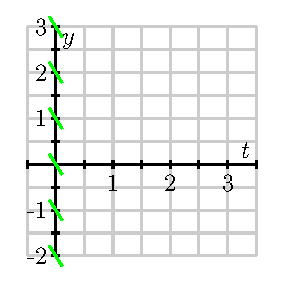
\includegraphics{figures/7_2_field_0.eps}
\end{center}
\caption{Beginnings of the slope field for $\ds \frac{dy}{dt} = t-2.$. }
\label{F:6.6_SF1}
\end{marginfigure}

Let's continue in the same way:  if $t=1$, the differential equation tells us that $dy/dt = 1-2=-1$, and this holds regardless of the value of $y$.  We now sketch tangent lines for several values of $y$ and $t=1$ with a slope of $-1$; see Figure~\ref{F:6.6_SF1}-(a).

%\begin{marginfigure} %MARGINFIGURE
%\begin{center}
%\subfloat[]{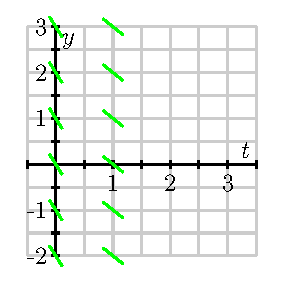
\includegraphics{figures/7_2_field_1.eps}}
%
%\subfloat[]{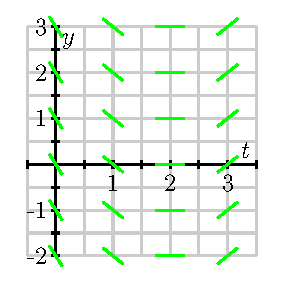
\includegraphics{figures/7_2_field_3.eps}}
%
%\subfloat[]{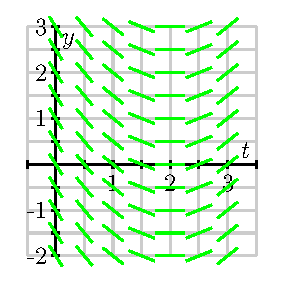
\includegraphics{figures/7_2_field_23a.eps}}
%\end{center}
%\caption{Generating the slope field for $\ds \frac{dy}{dt} = t-2.$.}
%\label{F:6.6_SF2}
%\end{marginfigure}

Similarly, we see that when $t=2$, $dy/dt = 0$ and when $t=3$, $dy/dt=1$.  We may therefore add to our growing collection of tangent line plots; see Figure~\ref{F:6.6_SF1}-(b). In this figure, you may see the solutions to the differential equation emerge.  However, for the sake of clarity, we will add more tangent lines to provide the more complete picture shown in Figure~\ref{F:6.6_SF2}-(c).

\begin{figure*} %MARGINFIGURE
\begin{flushright}
\subfloat[]{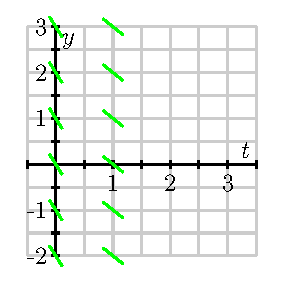
\includegraphics{figures/7_2_field_1.eps}}
\hspace{.5cm}
\subfloat[]{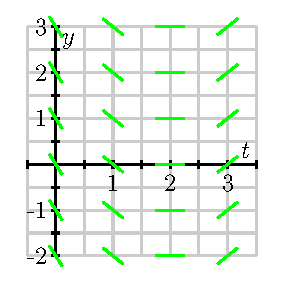
\includegraphics{figures/7_2_field_3.eps}}
\hspace{.5cm}
\subfloat[]{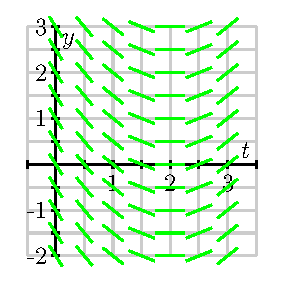
\includegraphics{figures/7_2_field_23a.eps}}
\end{flushright}
\caption{Generating the slope field for $\ds \frac{dy}{dt} = t-2.$.}
\label{F:6.6_SF2}
\end{figure*}

Figure~\ref{F:6.6_SF2}-(c) is called a {\em slope field}\index{slope field} for the differential equation, allows us to sketch solutions of the differential equation.  Here, we will begin with the initial value $y(0) = 1$ and start sketching the solution by following the tangent line, as shown in Figure~\ref{F:6.6_SF6}.

%\begin{marginfigure} %MARGINFIGURE
%\margingraphics{figures/7_2_field_30.eps}
%\caption{Sketching a solution curve for $\ds \frac{dy}{dt} = t-2.$. }
%\label{F:6.6_SF5}
%\end{marginfigure}

We then continue using this principle:  whenever the solution passes through a point at which a tangent line is drawn, that line is tangent to the solution.  Doing so leads us to the following sequence of images.

\begin{figure*} % MARGIN FIGURE
\begin{flushright}
\captionsetup[subfigure]{labelformat=empty}
\subfloat{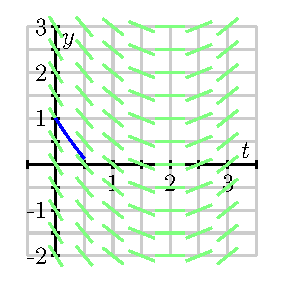
\includegraphics{figures/7_2_field_30.eps}}
\hspace{.25cm}
\subfloat{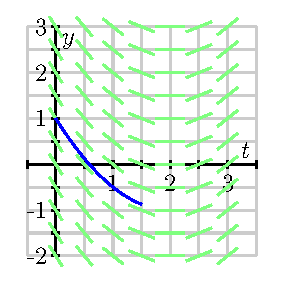
\includegraphics{figures/7_2_field_31.eps}}
\hspace{.25cm}
\subfloat{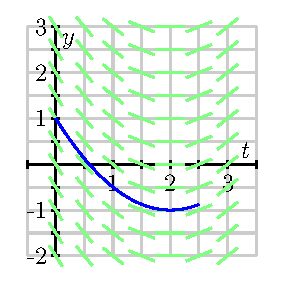
\includegraphics{figures/7_2_field_32.eps}}
\hspace{.25cm}
\subfloat{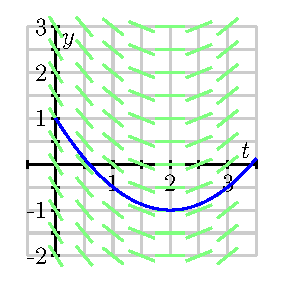
\includegraphics{figures/7_2_field_33.eps}}
\end{flushright}
\caption{Sketching a solution curve for $\ds \frac{dy}{dt} = t-2.$.}
\label{F:6.6_SF6}
\end{figure*}

In fact, we may draw solutions for any possible initial value, and doing this for several different initial values for $y(0)$ results in the graphs shown in Figure~\ref{F:6.6_SF7}.
 
Just as we have done for the most recent example with $\frac{dy}{dt} = t-2$, we can construct a slope field for any differential equation of interest.  The slope field provides us with visual information about how we expect solutions to the differential equation to behave.

\begin{marginfigure} %MARGINFIGURE
\begin{center}
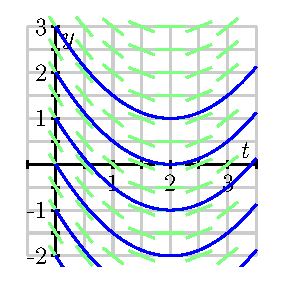
\includegraphics{figures/7_2_field_4.eps}
\end{center}
\caption{Several solution curves for $\ds \frac{dy}{dt} = t-2.$. }
\label{F:6.6_SF7}
\end{marginfigure}

\begin{activity} \label{A:6.6.4}  
  Consider the autonomous differential equation 
$$
\frac{dy}{dt} = -\frac 12( y - 4).
$$

\ba
\item Make a plot of $\frac{dy}{dt}$ versus $y$ on the axes provided.  Looking at the
  graph, for what values of $y$ does $y$ increase and for what values of $y$
  does $y$ decrease?

  \begin{center}
    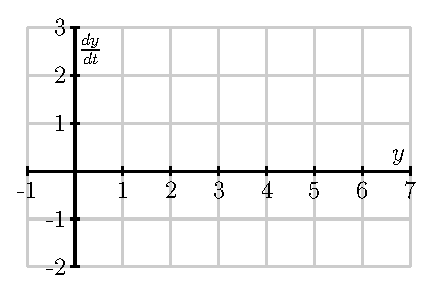
\includegraphics{figures/7_2_Act1_1.eps}
  \end{center}

\item Next, sketch the slope field for this differential equation on the axes provided.

  \begin{center}
    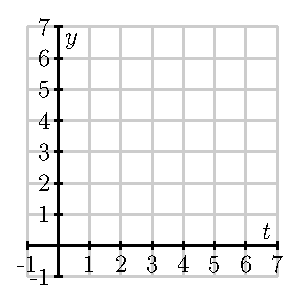
\includegraphics{figures/7_2_Act1_2.eps}
  \end{center}

\item  Use your work in (b) to sketch the solutions that satisfy $y(0) = 0$, $y(0) = 2$, $y(0) = 4$ 
  and $y(0) = 6.$

\item  Verify that $y(t) = 4 + 2e^{-t/2}$ is a solution to the given
  differential equation with the initial value $y(0) = 6.$  Compare
  its graph to the one you sketched in (c).

\item  What is special about the solution where $y(0) = 4$?  

\ea
\end{activity}
\begin{smallhint}
\ba
	\item Small hints for each of the prompts above.
\ea
\end{smallhint}
\begin{bighint}
\ba
	\item Big hints for each of the prompts above.
\ea
\end{bighint}
\begin{activitySolution}
\ba
	\item Solutions for each of the prompts above.
\ea
\end{activitySolution}
\aftera %ACTIVITY

%-----------------------------------------------------------
% SUBSECTION EQUILIBRIUM SOLUTIONS
%-----------------------------------------------------------
\subsection*{Equilibrium solutions and stability} 

As our work in Activity~\ref{A:6.6.4} demonstrates, first-order autonomous
solutions may have solutions that are constant.  In fact, these are
quite easy to detect by inspecting the differential equation $dy/dt =
f(y)$:  constant solutions necessarily have a zero derivative so 
$dy/dt = 0 = f(y)$.  

For example, in Activity~\ref{A:6.6.4}, we considered the
equation
$$
\frac{dy}{dt} = f(y)=-\frac12(y-4).
$$
Constant solutions are found by setting $f(y) = -\frac12(y-4) = 0$,
which we immediately see implies that $y = 4$.  

Values of $y$ for which $f(y) = 0$ in an autonomous differential equation $\frac{dy}{dt} = f(y)$ are usually called or {\em equilibrium solutions} \index{equilibrium solution} of the differential
equation.  

\begin{marginfigure}[6cm]
\margingraphics{figures/7_2_Act2_1.eps}
\end{marginfigure}

\begin{marginfigure}[1cm]
\margingraphics{figures/7_2_Act2_2.eps}
\end{marginfigure}

\begin{activity} \label{A:7.2.1}  
Consider the autonomous differential equation 
$$ \frac{dy}{dt} = -\frac 12 y(y-4). $$

\ba
\item Make a plot of $\frac{dy}{dt}$ versus $y$.  Looking at the
  graph, for what values of $y$ does $y$ increase and for what values of $y$
  does $y$ decrease?

\item Identify any equilibrium solutions of the given differential equation.

\item Now sketch the slope field for the given differential equation.

\item  Sketch the solutions to the given differential equation that correspond to initial values $y(0)=-1, 0, 1, \ldots, 5$.

\item  An equilibrium solution $\overline{y}$ is called {\em stable} \index{stable} \index{equilibrium solution!stable}
  if nearby 
  solutions converge to $\overline{y}$.  This means that if the inital
  condition varies slightly from $\overline{y}$, then
  $\lim_{t\to\infty}y(t) = \overline{y}$.  

  Conversely, an equilibrium solution $\overline{y}$ 
  is called {\em unstable} \index{unstable} \index{equilibrium solution!unstable} if nearby solutions are pushed away from
  $\overline{y}$.

  Using your work above, classify the equilibrium solutions you found in (b)
  as either stable or unstable.

\item Suppose that $y(t)$ describes the population of a species of
  living organisms and that the initial value $y(0)$ is positive.  What can you
  say about the eventual fate of this population?  

\item  Remember that an equilibrium solution $\overline{y}$ satisfies
  $f(\overline{y}) = 0$.  If we graph $dy/dt = f(y)$ as a function of
  $y$, for which of the following differential equations is
  $\overline{y}$ a stable equilibrium and for which is $\overline{y}$ unstable?  Why?

  \begin{center}
    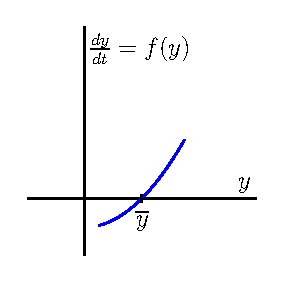
\includegraphics{figures/7_2_Act2_3.eps} \qquad
    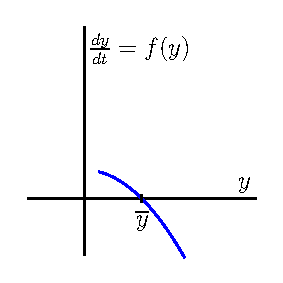
\includegraphics{figures/7_2_Act2_4.eps} 
  \end{center}

\ea
\end{activity}
\begin{smallhint}
\ba
	\item Small hints for each of the prompts above.
\ea
\end{smallhint}
\begin{bighint}
\ba
	\item Big hints for each of the prompts above.
\ea
\end{bighint}
\begin{activitySolution}
\ba
	\item Solutions for each of the prompts above.
\ea
\end{activitySolution}
\aftera %ACTIVITY

%---------------------------------------------
% SUMMARY
%---------------------------------------------
\begin{summary}
\item A differential equation is simply an equation that describes the
  derivative(s) of an unknown function.
\item Physical principles, as well as some everyday situations, often
  describe how a quantity changes, which 
  lead to differential equations.
\item A solution to a differential equation is a function whose
  derivatives satisfy the equation's description.  Differential
  equations typically have infinitely many solutions, 
  parameterized by the initial values.
\item A slope field is a plot created by graphing the tangent lines of
  many different solutions to a differential equation.
\item Once we have a slope field, we may sketch the graph of solutions
  by drawing a curve that is always tangent to the lines in the slope
  field. 
\item Autonomous differential equations sometimes have constant
  solutions that we call 
  equilibrium solutions.  These may be classified as stable or
  unstable, depending on the behavior of nearby solutions.  
\end{summary}

\clearpage

%--------------
% EXERCISES
%--------------
\begin{adjustwidth*}{}{-2.25in}
\textbf{{\large Exercises}}
\setlength{\columnsep}{25pt}
\begin{multicols*}{2}

\noindent {\normalsize Problems} \small

\begin{enumerate}[1)]
 \item Suppose that $T(t)$ represents the temperature of a cup of
    coffee set out in a room, where $T$ is expressed in degrees
    Fahrenheit and $t$ in minutes.  A physical principle known as    Newton's Law of Cooling\index{Newton's Law of Cooling} tells us that 
    $$
    \frac{dT}{dt}= -\frac1{15}T+5.
    $$

\ba
    \item Supposes that $T(0)=105$.  What does the differential
    equation give us for the value of $\ds \frac{dT}{dt}\vert_{T=0}$?  Explain in a
    complete sentence the meaning of these two facts.

    \item Is $T$ increasing or decreasing at $t=0$?

    \item What is the approximate temperature at $t=1$?

    \item On the graph below, make a plot of $dT/dt$ as a function of $T$.
        \begin{center}
          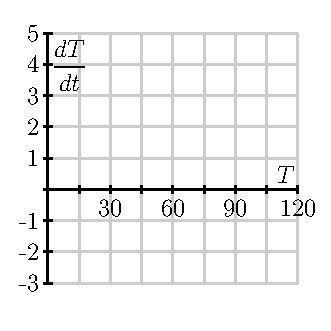
\includegraphics{figures/7_1_exercise_1.eps}
        \end{center}

       \item For which values of $T$ does $T$ increase?  For
        which values of $T$ does $T$ decrease?

        \item What do you think is the temperature of the room?
        Explain your thinking.

        \item Verify that $T(t) = 75 + 30e^{-t/15}$ is the
        solution to the differential equation with initial value $T(0)
        = 105$.  What happens to this solution after a long time?
  \ea
  
  \item Suppose that the population of a particular species is
    described by the function $P(t)$, where $P$ is expressed in
    millions.  Suppose further that the population's rate of change is
    governed by the differential equation 
    $$\frac{dP}{dt} = f(P)
    $$
    where $f(P)$ is the function graphed below.

    \begin{center}
      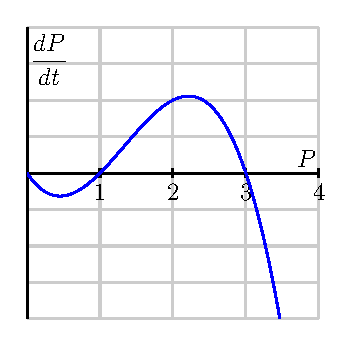
\includegraphics[scale=.75]{figures/7_1_threshold.eps}
    \end{center}

\ba
    \item For which values of the population $P$ does the population
      increase?

      \item For which values of the population $P$ does the population
      decrease? 

      \item  If $P(0) = 3$, how will the population change in time?

     \item  If the initial population satisfies $0<P(0)<1$, what will
      happen to the population after a very long time?

      \item  If the initial population satisfies $1<P(0)<3$, what will
      happen to the population after a very long time?

      \item If the initial population satisfies $3<P(0)$, what will
      happen to the population after a very long time?

      \item  This model for a population's growth is sometimes called
      ``growth with a threshold.''  Explain why this is an appropriate
      name.  

\ea

  \item In this problem, we test further what it means for a function to be a solution to a given differential equation.
  \ba
  	\item Consider the differential equation
      $$
      \frac{dy}{dt} = y - t.
      $$
      Determine whether the following functions are solutions to the given differential equation.

      \begin{itemize}
 	\item[(i)] $y(t) = t + 1 + 2e^t$
	\item[(ii)] $y(t) = t + 1$
	\item[(iii)] $y(t) = t + 2$
       \end{itemize}

	\item   When you weigh bananas in a scale at the grocery store, the
      height $h$ of the bananas is described by the differential
      equation
      $$
      \frac{d^2h}{dt^2} = -kh
      $$
      where $k$ is the {\em spring constant}, a constant that depends
      on the properties of the spring in the scale.  After you put the
      bananas in the scale, you (cleverly) observe that the height of the bananas
      is given by $h(t) = 4\sin(3t)$.  What is the value of the spring
      constant? 
    \ea
        
\end{enumerate}

%------------------------------------------
% END OF EXERCISES ON FIRST PAGE
%------------------------------------------
\end{multicols*}
\end{adjustwidth*}

\afterexercises 

\cleardoublepage
